%!TEX root = ../template.tex
%%%%%%%%%%%%%%%%%%%%%%%%%%%%%%%%%%%%%%%%%%%%%%%%%%%%%%%%%%%%%%%%%%%%
%% chapter3.tex
%% NOVA thesis document file
%%
%% Chapter with a short latex tutorial and examples
%%%%%%%%%%%%%%%%%%%%%%%%%%%%%%%%%%%%%%%%%%%%%%%%%%%%%%%%%%%%%%%%%%%%

\typeout{NT FILE chapter3.tex}%

\chapter{Architecture}
\label{cha:architecture}

\paragraph{}In this chapter there will be a presentation of the architecture of the proposed solution as well as some insights into its 
implementation.

\section{System Overview}
\label{sec:systemoverview}
\paragraph{}The proposed solution is designed to address the complexities of navigating a 
tractor-trailer system in narrow environments, such as agricultural fields. This system integrates 
advanced path planning and control strategies to ensure safe practices, with collision avoidance, and 
effective navigation, tending to the specific needs of this type of system.

The system is divided into two main components: a self-propelled tractor and a non-propelled trailer. 
The tractor is an Agilex Scout V2 which is a four-wheeled differential driven robot that serves as the 
navigation an propulsion unit. The trailer, designed for modularity can have its own independent functionalities 
allowing for a simpler maintenance and adaptability to different tasks. This modullarity allows 
for the independant development of the tractor's navigation and control systems without 
the need of knowing the trailer's payload or functionalities, with perhaps the exception 
of the trailer hindering the sensor's view or the trailer's weight exceeding the 
tractor's capabilities.

The solution proposed in this work is divided into four main modules:
\begin{itemize}
    \item \textbf{Environment}: This module is responsible for the representation of the real world, or actually be the real world. This is where the robot will operate.
    \item \textbf{Sensor perception}: This module is responsible for gathering data from the environment and converting it into usable information like localization and estimation.
    \item \textbf{Path planning}: This module is responsible for generating a feasible path from the current position to the desired goal.
    \item \textbf{Control}: This module is responsible for tracking the generated path and ensuring the tractor-trailer system follows it safely without collisions.
\end{itemize}

From the modules mentioned above, the ones that are implemented in this work are mainly 
the path planning and control modules, however, in order to test and develop the system, 
the environment and sensors were simulated.

The overall functioning of the system is as follows: the tractor is at a point in the environment, simulation or real world, 
the user then requests a movement to a specific position, the path planning module will then generate a path from the current 
position, estimated with sensor gathered data, to the desired goal. The path is then forwarded to the 
controller which will then track it by computing the necessary angular and linear velocities while ensuring the 
physical constraints of the tractor-trailer system are respected.
 

% insert figure with an uml diagram of the syste architecture

\section{Hardware}
\label{sec:hardware}

\paragraph{}The tractor used is an Agilex Scout which is a four wheeled differential driven robot, 
equipped with a NVIDIA Jetson Agx Xavier as the main computer, a LIDAR and wheel decoders. 
the NVIDIA Jetson Agx Xavier is a powerful computer capable of running complex algorithms in real time, 
and is used to run the whole system, from path planning to control and sensor 
perception. The Lidar and decoders are used to gather data for localization and mapping. This 
robot can be teleoperated using a controller, or can be programmed 
to do whatever autonomous task is requiered since all its instruments 
are accessible in the Jetson Agx Xavier. The tractor is shown in the figure below:

\begin{figure}[h]
    \centering
    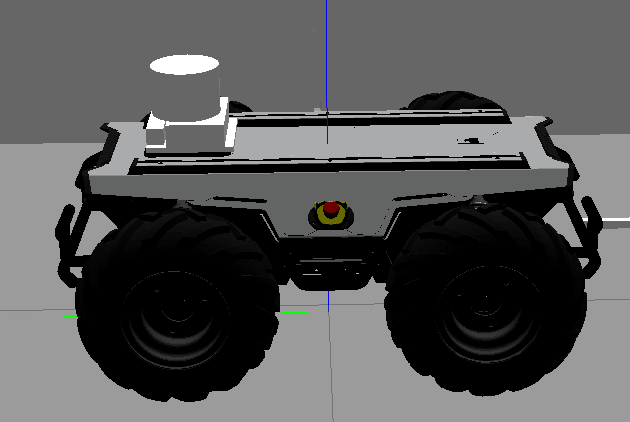
\includegraphics[width=0.75\textwidth]{tractor_gazebo.png}
    \caption{Simulated tractor in Gazebo.}
\end{figure}

There's no representation of the jetson in the simulation since the program is running on 
the same machine as the simuation. However, it is possible to 
notice the Lidar rack on top of the other instruments. Once again, this is 
but a representation for simulation purposes, as the real tractor has a similar 
configuration, shown in figure \ref{fig:tractor}.
\begin{figure}[h]
    \centering
    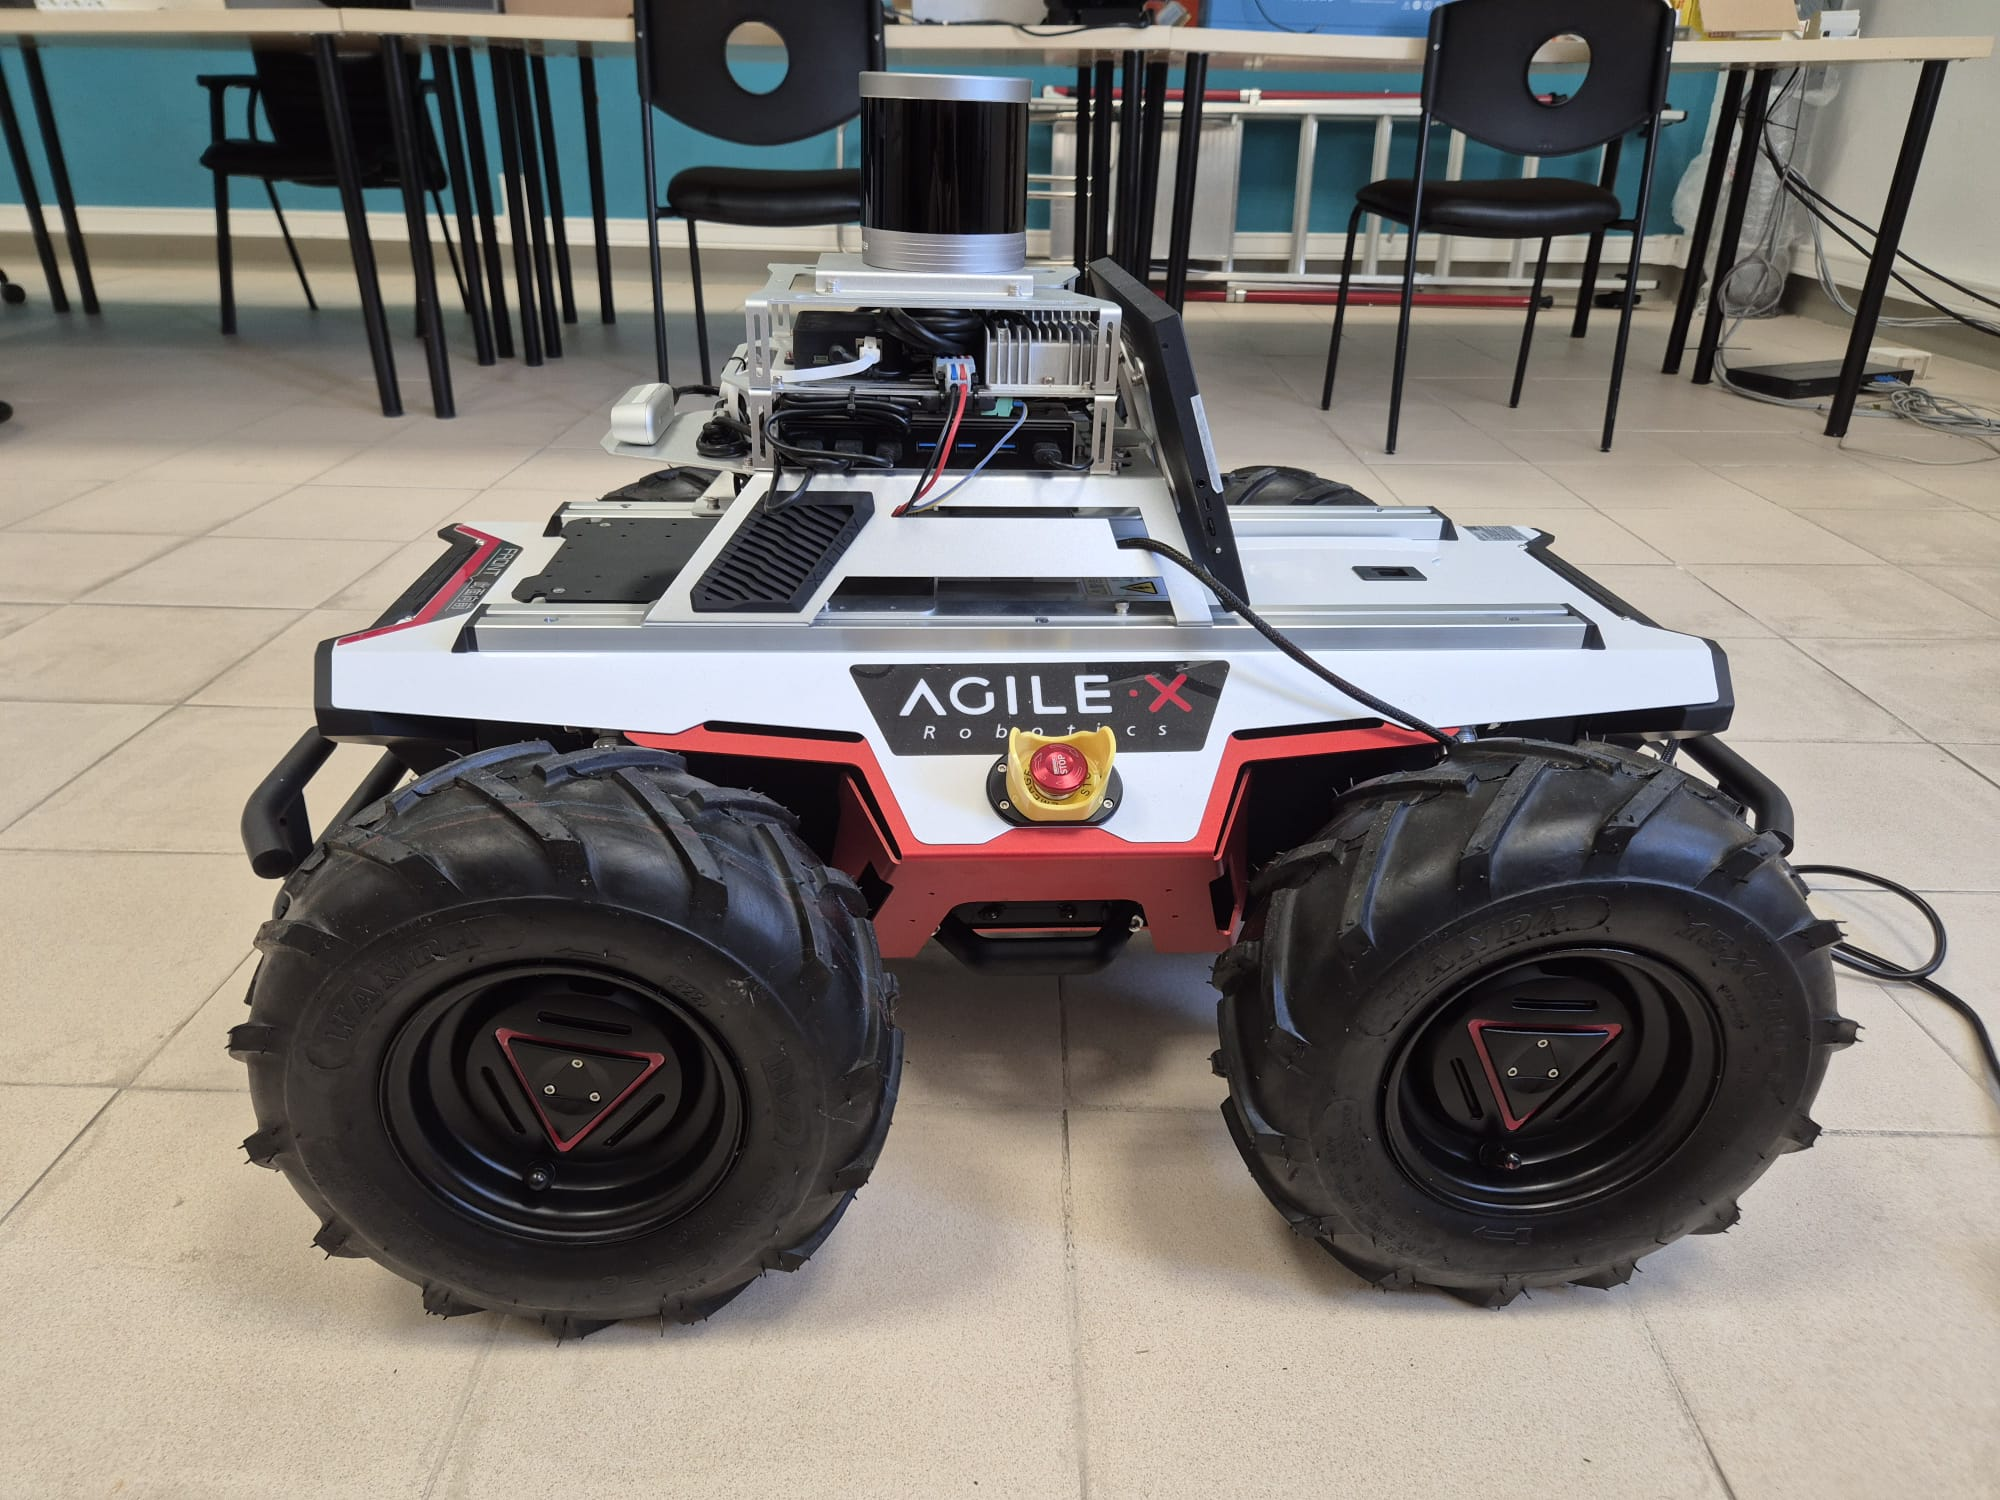
\includegraphics[width=0.75\textwidth]{tractorreal.jpg}
    \caption{Real tractor.}
    \label{fig:tractor}
\end{figure}

 
\begin{figure}[h]
    \centering
    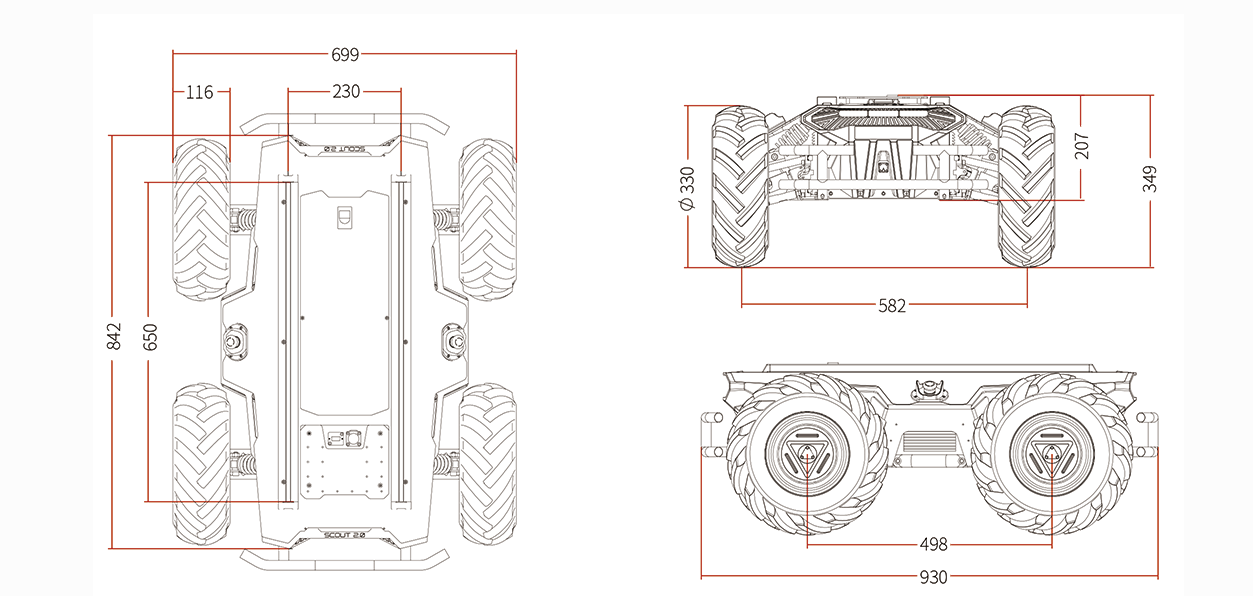
\includegraphics[width=0.9\textwidth]{tractordim.png}
    \caption{Agilex Scout dimensions \cite{scoutdim}.}
    \label{fig:tractordim}
\end{figure}

The figures \ref{fig:tractordim} and \ref{fig:tractor} show the robot, its dimensions, and also the 
the additional rack, at the top, where the computer, Lidar and all other required electronics 
are mounted.

Additionally, the tractor is pulling a trailer, which is equipped with 
a spray system, however for the sake of simplicity, to test the navigation 
and control algorithms, the tests were be done with the following trailer:
\clearpage
\begin{figure}[h]
    \centering
    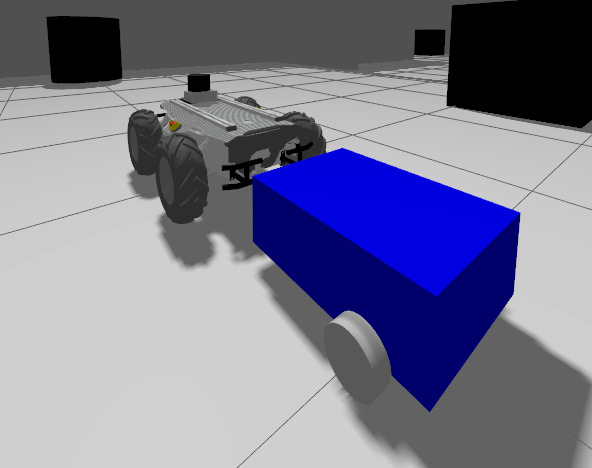
\includegraphics[width=0.75\textwidth]{trailergazebo.jpg}
    \caption{Tractor-trailer system simulated in Gazebo Classic.}
    \label{fig:trailergazebo}
\end{figure}

The trailer shown in figure \ref{fig:trailergazebo}, is a representation of a generic trailer, not having any specific 
functions other than following the systems dynamics, which is the main focus of this work. 
One particular aspect of this robot is that there's no sensor for 
trailer position and, therefore, it is estimated in real time using the 
system's dynamics shown in \ref{subsec:SD}.
\section{Planner}
\label{sec:planner1}
\paragraph{}The planner is a Voronoi Hybrid A* mixture which takes the 
ability to generate feasible paths from the Hybrid A* and the 
added velocity of having a pre-computed Voronoi graph to expand 
from.

The following flowchart shows the logic of the planner, starting with 
the request for movement, assigning a goal target. Then, the planner will 
preform an A* search on the pre computed Voronoi Graph, starting from the current robot 
positon, to the goal pose. The A* search will return a path which consists 
of a series of subgoals which will later on be used to speed up the 
path creation process. Having the subgoals, the next step is to try and 
find a feasible path from the current position to the subgoal nearest to 
the goal pose, in this case, since it is the first iteration, the actual goal. 
If the path is feasible, then the planner will simply return said path, otherwise
 the planner will try to do the same but with the next subgoal, until it either finds 
a feasible path or exhausts all the subgoals. If it finds a path, it will 
repeat the previous process, but instead of using the current position as the 
starting configuration, it will use the subgoal which a path was able to be 
computed to. If it exhausts all the subgoals, then it will try and compute a new node, 
a Hybrid A* node, which consists of a segment, starting from the current algorithmic position 
(can be the start point or a subgoal depending if a path was found previously), to any point 
that is reachable by the tractor at a distance $d$ defined by the user, and then assign them as the 
current algorithmic position to run the Dubins loop again.
\begin{figure}[h]
    \centering
    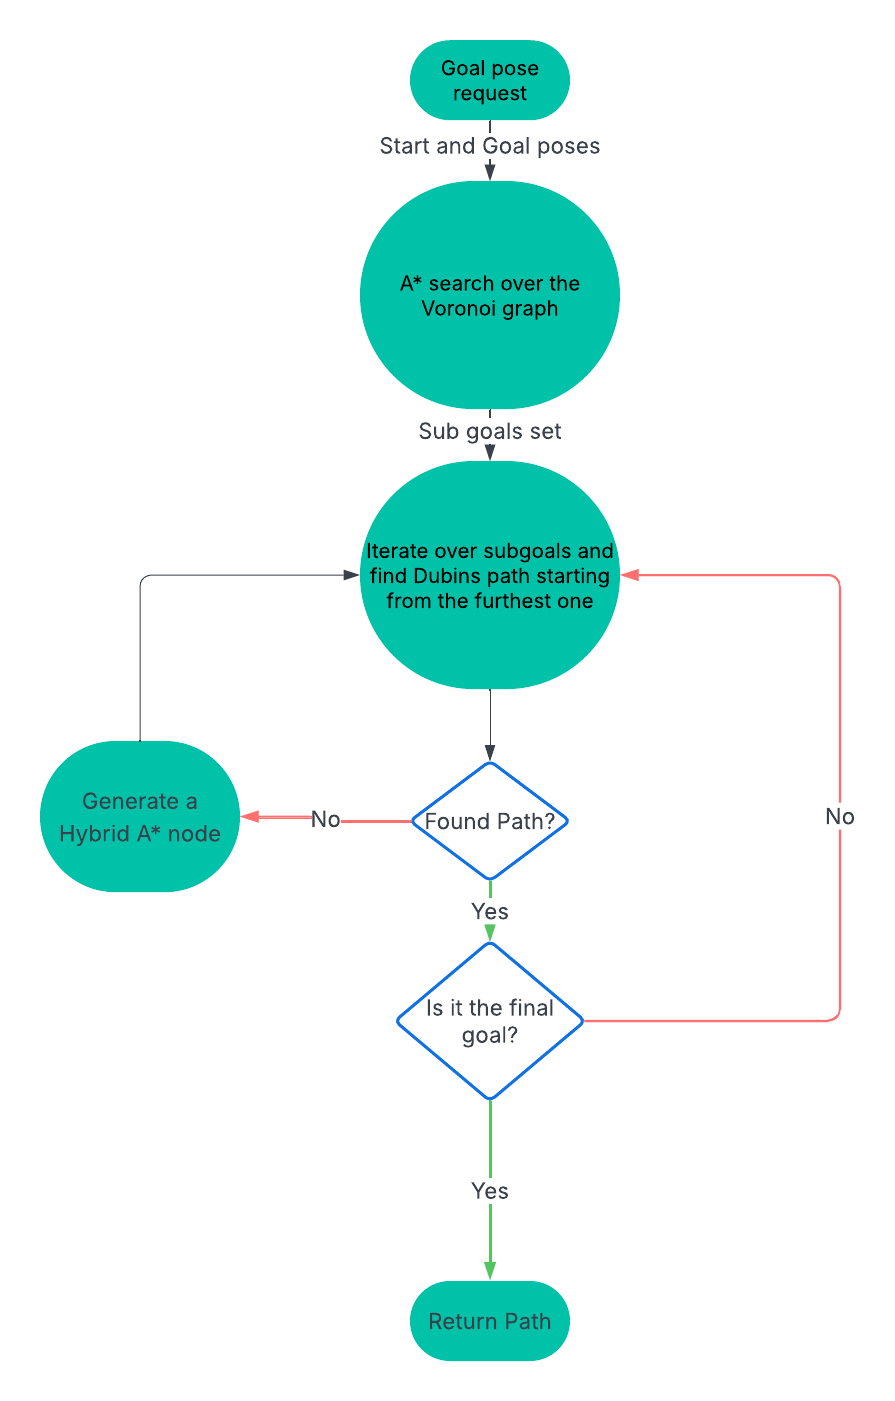
\includegraphics[width=0.85\textwidth]{Flowchart.png}
    \caption{Planner logic flowchart}
\end{figure}

\begin{algorithm}
\caption{Planner Pseudocode}
\label{alg:planner}
\begin{algorithmic}[1]
\Function{get\_path}{start, goal}
    \State subgoals $\gets$ get\_subgoals(start, goal, voronoi\_graph)

    \State current $\gets$ start

    \State path $\gets$ None
    \ForAll{subgoal in subgoals}
        \State path $\gets$ get\_feasible\_path(path, current, subgoal)
        \If{path $\neq$ None}
            \If{subgoal $=$ goal}
                \State \Return path
            \Else
                \State current $\gets$ subgoal
            \EndIf
        \EndIf
    \EndFor
    \While{True}
        \State new\_node $\gets$ expand\_hybrid\_node(start)
        \If{check\_not\_feasible(new\_node)}
            \State \Return None
        \EndIf
        \State path $\gets$ attatch\_node\_to\_path(path,new\_node, goal)
        \State current $\gets$ new\_node
    \EndWhile
\EndFunction
\end{algorithmic}
\end{algorithm}

The algorithm \ref{alg:planner} shows the detailed pseudocode for the planner. Starting 
with the subgoals generation, to the looping through them and trying to find a path, 
to, if needed, the expansion of the hybrid A* nodes.
\begin{algorithm}[h]
\caption{Get\_subgoals Pseudocode}
\label{alg:get_subgoals}
\begin{algorithmic}[1]
\Function{get\_subgoals}{start, goal, voronoi\_graph}
    \State subgoals $\gets$ []
    \State closed\_list $\gets$ []
    \State open\_list $\gets$ [start]
    \State found $\gets$ False

    \While{open\_list.not\_empty() and not found}
        \State current $\gets$ open\_list.pop()
        \State closed\_list.append(current)
        \State neighbours $ \gets$ current.neighbours
        \ForAll{neighbour in neighbours}
            \If{neighbour not in closed\_list} 
                \If{neighbour in open\_list}
                    \If{current.f < open\_list(neighbour).f}
                        \State continue
                    \EndIf
                \EndIf
                \State current.parent $\gets$ current
                \State current.f $\gets$ compute\_fcost(current, neighbour, goal)
                \State open\_list.append(neighbour)
            \EndIf
            \If{neighbour is goal}
                \State goal.parent $\gets$ current 
                \State found $\gets$ True
                break
            \EndIf
        \EndFor
    \EndWhile
    \If{found}
        \State current $\gets$ goal
        \While{current is not start}
            \State subgoals.append(current)
            \State current $\gets$ current.parent
        \EndWhile
    \EndIf
    \State \Return subgoals
\EndFunction
\end{algorithmic}
\end{algorithm}

Algorithm \ref{alg:get_subgoals} shows the pseudocode for the subgoal generation, 
which is done by performing a regular A* search on the pre-computed Voronoi graph. 
It starts by examining the neighbours of the start node and adding them 
to the open list, it then goes through the open list and preforms the 
same operation until the goal is found or the open list is empty.

The Dubins path creation is more mathmatically complex to represent simply in pseudocode. 
It is a calculation of forwards segments that can be of 6 different types, 
Left Straight Left (LSL), Left Straight Right (LSR), Right Straight Left (RSL), Right Straight Right (RSR), 
Right Left Right (RLR) and Left Right Left (LRL). These paths are the shortest possible 
curves connecting two configurations for a non-holonomic vehicle with a fixed minimum radius.
The process is devided into six main steps, normalizing the problem, byt calculating the 
distances between start and goal configurations and also the orientation, the start 
heading from start to goal and the goal heading relative to the line connecting the start and goal. 
the next step is to compute the six paths, one of each type and check their feasibility, then, 
the feasible paths are sorted by length and the shortest is the chosen one. Finally, 
the path is then segmented into short segments of ($x$,$y$ and $yaw$) and then returned.
\begin{algorithm}[h]
\caption{Expand\_hybrid\_node Pseudocode}
\label{alg:expand_hybrid_node}
\begin{algorithmic}[1]
\Function{expand\_hybrid\_node}{node, open\_list, directions, node\_length}
    \ForAll {sign in \{-1, 1\}}
        \ForAll{d in directions}
            \State segment $\gets$ [node.x, node.y, node.yaw]
            \For i in node\_length
                \State new\_node $\gets$ new\_node()
                \State new\_node.yaw $\gets$ segment.last.yaw + d
                \State new\_node.x $\gets$ sign * segment.last.x + i * cos(new\_node.yaw)
                \State new\_node.y $\gets$ sign * segment.last.y + i * sin(new\_node.yaw)
                \State new\_node.parent $\gets$ segment.last.parent
                \State new\_node.f $\gets$ compute\_fcost(new\_node, goal)
                \State segment.append(new\_node)
            \EndFor
            \If{check\_feasibility(new\_node)}
                \State open\_list.append(new\_node)
            \EndIf
        \EndFor
    \EndFor
\EndFunction
\end{algorithmic}
\end{algorithm}

The algorithm \ref{alg:expand_hybrid_node} shows the pseudocode for the hybrid A* node expansion. It first 
iterates through all the parameterised directions (steering angles), and creates 
segments of the tractor's movement, forwards and backwards. All these segments are checked for 
feasibility, which is done by verifying if the trailer is not colliding with the tractor or 
with any obstacles in the environment. The feasible segments are then added to open list to be used 
in the next iteration of the planner and verify if a Dubins path is feasible from that new position.
\begin{figure}[h]
    \centering
    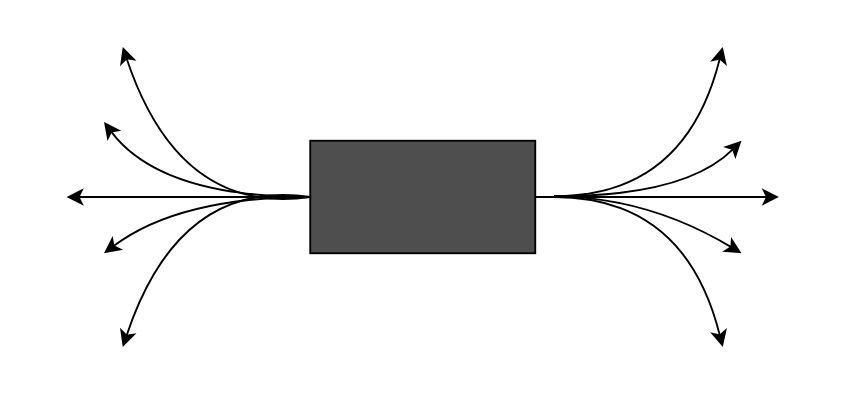
\includegraphics[width=0.6\textwidth]{hybridnodeexpansion.png}
    \caption{Hybrid A* node expansion.}
    \label{fig:hybridnodeexpansion}
\end{figure}

In figure \ref{fig:hybridnodeexpansion}, the rectangle represents the tractor and the 
arrows the segments created, forwards and backwards, representing the recovery process. 
The amount of nodes, length of the segments and the maximum radius can be parameterised by the user, 
allowing for more diversity of operatioal environments.

\section{Controller}
\label{sec:controller}
\paragraph{}A path is nothing if it cannot be followed so, a controller capable of 
attending to this system's needs is required. This controller will 
receive as input the generated path by the planner and will try to track it. 
This is achieved in two steps, first, having the current positions in mind, 
it will choose the next subgoal in the path. Since the controller is 
a \gls{PP} controller, the subgoal is chosen depending on the lookahead distance, 
as explained in \ref{subsec:PP}. The next step is to compute the angular velocity needed 
for the robot to reach said subgoal. For this, two controllers were used:
\begin{itemize}
    \item \textbf{Forwards Controller}: Used when the tractor is moving forwards.
    \item \textbf{Backwards Controller}: Used when the tractor is moving backwards.
\end{itemize}
The choice of controller depends on the orientation of the tractor and 
direction to the next subgoal. The need for two controllers arises from 
the fact that when moving backwards, the movement needs to be optimised 
for the trailer's position and orientation, while when moving forwards, 
the movement needs only to be optimised for the tractor's movement as the 
trailer positions are move predictable when moving forwards.

The forwards controller is defined by the following equations:
\begin{equation}
    \omega = \tan^{-1}\left(\frac{2*WB*sin(\epsilon_{\theta_0})}{l_f}\right)
\end{equation}
where $WB$ is the wheelbase of the tractor, $l_f$ is the lookahead distance and 
$\epsilon_{\theta_0}$ is the error in the angle between the tractor and the next goal.
\begin{equation}
    \epsilon_{\theta_0} = \tan^{-1}\left(\frac{t_y - y_r}{t_x - x_r}\right) - \theta_0
\end{equation}
The $t_x$ and $t_y$ are target point coordinates and $x_r$ and $y_r$ are the current tractor center coordinates. 
As explained previously, this controller only cares about the tractor's 
configuration, which makes having a feasible path all the more important.

The backwards controller, on the other hand, is defined by the following equations:
\begin{equation}
    \omega = V \left(-k (\theta_1 - \alpha^*) - \frac{sin\theta_1}{RTR}\right)
\end{equation}
where $RTR$ is the distance between the hitch joint and the trailer's real axle, 
$k$ is a constant, $\theta_1$ is the angle between the tractor and the trailer, 
$V$ is the linear velocity of the tractor and 
\begin{equation}
    \alpha^* = tan^{-1}\left(\frac{2*RTR*sin(\epsilon_{\theta_1})}{l_f}\right)
\end{equation}
with
\begin{equation}
    \epsilon_{\theta_1} = \tan^{-1}\left(\frac{t_y - y_t}{t_x - x_t}\right) - \theta_t
\end{equation}
where $t_x$ and $t_y$ are the target point coordinates and $x_t$ and $y_t$ are the current trailer real axle coordinates and 
$\theta_t$ is the orientation of the trailer. It is observed that 
these equations are similar to the forwards controller, however, they differ 
in the fact that the goal pose is defined by the trailer's position. Even though 
this controller is taking the trailer's constraints into account, due to 
the inate nature of the tractor-trailer system being non-holonomic, the 
path planner is still the one responsible for maintaining the feasibility 
of the movement.


\section{Collision Avoidance}
\label{sec:collision}
The collision avoidance aspect of the controller is of the utmost importance 
in real world scenarios when dealing with possible workers in the field. To achieve 
this safety requirement, the controller is equipped with a collision detection algorithm 
which will check for obstacles in the way of the tractor-trailer system and remain still until the 
obstacle is no longer in the way or another path update has been sent.

The algorithm works by calculating the angle between the tractor and the chosen 
subgoal in the path, then, it will check if there are any obstacles in the rectangle 
created along the line connecting the tractor and subgoal. If true, the controller will 
give signal that a collision is imminent and commands will be to stop and wait.

\begin{figure}[h]
    \centering
    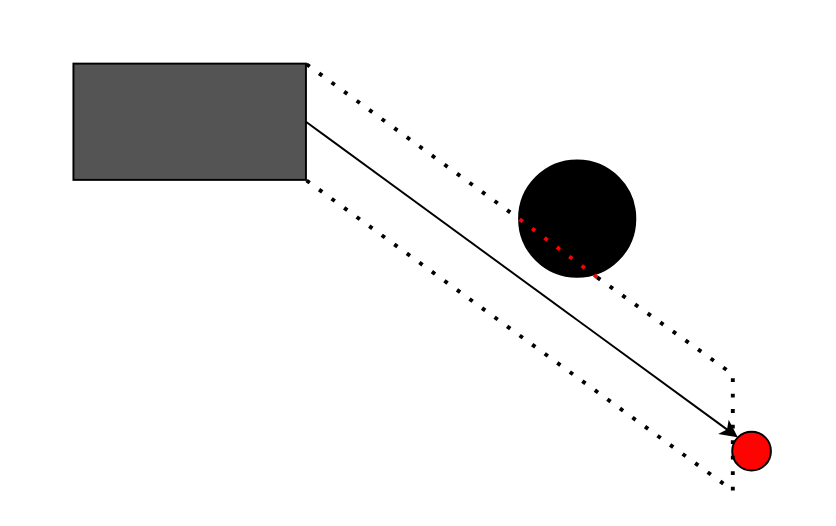
\includegraphics[width=0.6\textwidth]{collisiondetection.png}
    \caption{Representation of the collsion detection module. In red the goal pose, in grey the tractor, the black circle is the obstacle and then the doted rectangle the expanded rectangle used to check for collisions.}
    \label{fig:collisiondetection}
\end{figure}

\section{Final Architecture}
\label{sec:final_architecture}

\paragraph{}The final architecture acn be seen in figure \ref{fig:system_architecture}, 
where the modules are represented and how they interact with each other. The environment is either 
the real world or a simulated world totaly created form scratch, the sensors are the Lidar and Wheel encoders, 
which are represented by the real word counterparts or gazebo plugins. The Extended Kalman Filter is 
used to estimate the tractor's transform using the wheel speed from the encoders and is an available 
package from the \gls{NAV2} framework. The map that is in the Map server has to be created manually using 
\gls{SLAM}. The \gls{AMCL} node is available inside the \gls{NAV2} framework and is used to localize the tractor given the map and a Laser scan. 
The point cloud to laser scan library used needed to be configured to work with the tractor's 3D LIDAR. 
The BT Navigator server is part of the \gls{NAV2} framework. The planner server is using a totally 
custom plugin, made from scratch that is used to get the Global Plan from the start and goal poses. The 
controller server is also using a totally custom plugin, made from scratch, that is used to get 
the velocities for forwards and backwards movements as well as the collision detection to stop the tractor. 



\begin{figure}[h]
    \centering
    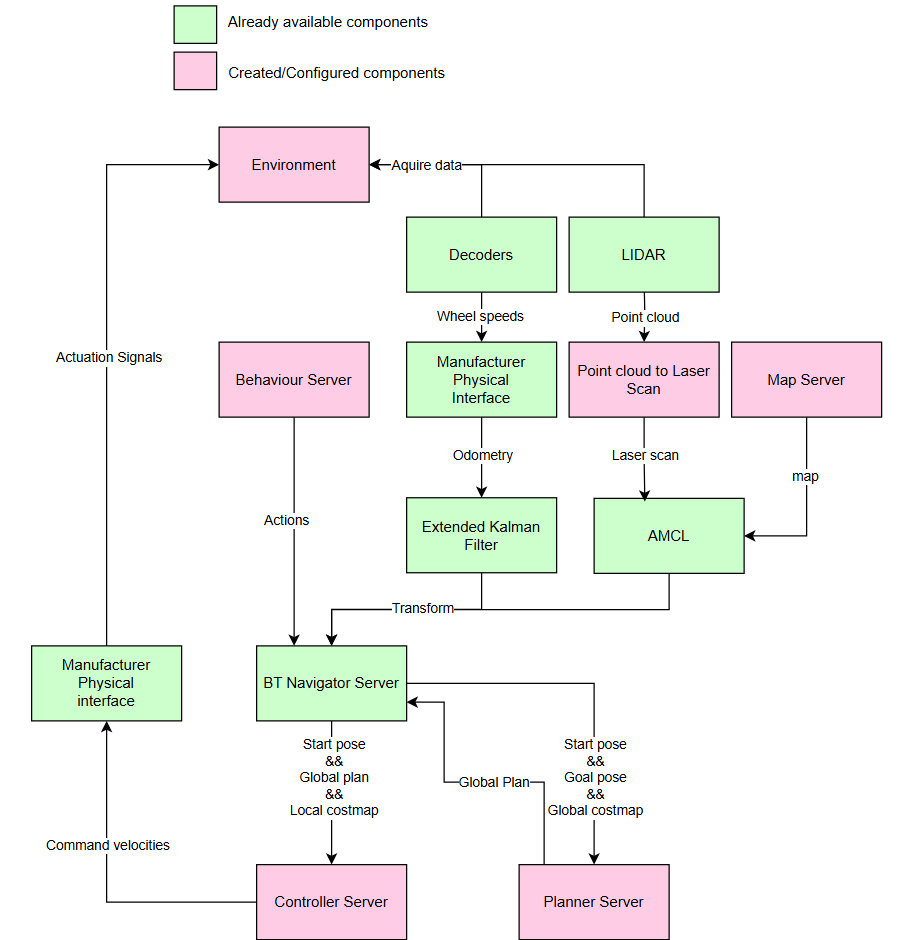
\includegraphics[width=0.95\textwidth]{systemarchitecture.png}
    \caption{System architecture overview. In pink are the components that have been completely implemented or configured, and in green the already available components from either NAV2, ROS2 or even the manufacturers.}
    \label{fig:system_architecture}
\end{figure}
